\documentclass[11pt,a4paper]{article}

\usepackage[utf8]{inputenc}
\usepackage[top=0.85in,bottom=0.85in,left=0.85in,right=0.85in]{geometry}
\usepackage{amsmath,amssymb,amsfonts}
\usepackage{booktabs}
\usepackage{graphicx}
\usepackage{tikz}
\usetikzlibrary{shapes.geometric, arrows.meta, positioning, calc}
\usepackage{hyperref}
\usepackage{cite}
\usepackage{array}
\usepackage{microtype}
\usepackage{tabularx}
\usepackage{enumitem}

\hypersetup{
    colorlinks=true,
    linkcolor=blue!80!black,
    citecolor=blue!80!black,
    urlcolor=blue!80!black
}

% Tight spacing controls to guarantee <= 10 pages in Overleaf
\setlength{\parskip}{0.3em}
\setlength{\parindent}{1.2em}
\renewcommand{\topfraction}{0.85}
\renewcommand{\bottomfraction}{0.85}
\renewcommand{\textfraction}{0.15}
\renewcommand{\floatpagefraction}{0.8}

% Compact bibliography formatting
\let\oldthebibliography\thebibliography
\let\endoldthebibliography\endthebibliography
\renewenvironment{thebibliography}[1]{
  \begin{oldthebibliography}{#1}
    \setlength{\itemsep}{0.15em}
    \setlength{\parskip}{0em}
}
{
  \end{oldthebibliography}
}

\begin{document}

% -------------------------------------------------------------------------
% Title & Authors (Template Structure)
% -------------------------------------------------------------------------
\begin{center}
    {\LARGE \textbf{KALANTAR: An Explainable and Probabilistic AI-Based Railway Intelligence System for Dynamic Train ETA Prediction, Delay Propagation Analysis, and Passenger Decision Support}}
    \vspace{1.0em}

    \textbf{Harsh}$^{*}$ (Reg. No. 12311856), \textbf{Charan Teja} (Reg. No. 12311893), \textbf{Chityala Vishal} (Reg. No. 12311775), \\
    \textbf{Anshul Jain} (Reg. No. 12311864), and \textbf{Abhi Raj Nigam} (Reg. No. 12307536)
    \vspace{0.5em}

    Department of Computer Science and Engineering, Lovely Professional University, Phagwara, Punjab 144411, India \\
    \vspace{0.3em}
    $^{*}$Correspondence to: Harsh, Registration No. 12311856, Department of Computer Science and Engineering, Lovely Professional University, Phagwara, Punjab 144411, India; Email: \texttt{harsh12311856@gmail.com}
\end{center}

\vspace{0.5em}

% -------------------------------------------------------------------------
% Abstract
% -------------------------------------------------------------------------
\noindent\textbf{Abstract} \\
Trains in large national networks rarely run in isolation. When one service stalls, the knock-on effects quickly ripple across shared junctions, track blocks, and turnaround platforms. Current railway tracking apps tell passengers only that a train is running late, offering a single static arrival time without any confidence interval and without checking if the passenger will miss their connecting train at the next junction. In this project, we built and tested \textbf{KALANTAR}, an end-to-end railway intelligence system that solves these gaps. We split 1.5 million synthetic Indian rail journey records chronologically from 2018 to 2024 and trained an XGBoost model to predict arrival delays. On our unseen 2024 test data, the model achieved a Mean Absolute Error of 34.92 minutes, beating standard median baselines by 33.2\%. We used TreeSHAP to interpret individual predictions and derived an empirical 80\% confidence interval of $[-53.4\,\mathrm{min}, +58.8\,\mathrm{min}]$ around each forecast. When we audited the physical network using 186,114 cleaned timetable rows across 8,151 stations, we discovered a massive 355.25~km median distance mismatch between journey logs and timetable entries across 1,820 common train numbers. Instead of forcing a flawed dataset join, we built a decoupled simulation pipeline: the machine learning model estimates initial journey delays, while an independent 175,002-edge timetable graph simulates station buffer absorption, evaluates passenger connection risks, and recommends alternate trains when transfers fail. We packaged the entire pipeline into a FastAPI service running on port 8050 with an interactive web dashboard.

\vspace{0.5em}
\noindent\textbf{Keywords} \\
Alternative Routing, Buffer Absorption, Decision Support Systems, Delay Propagation, Estimated Time of Arrival, Explainable AI, Graph Modeling, Indian Railways, Intelligent Transportation, Probabilistic Forecasting, Rake Turnaround, SHAP, Timetable Resilience, Uncertainty Quantification, XGBoost.

\vspace{0.8em}

% -------------------------------------------------------------------------
% 1. Introduction
% -------------------------------------------------------------------------
\section{Introduction}

Anyone who has traveled on Indian Railways knows that train delays are routine. The network carries over 22 million passengers every single day across 68,000 route kilometers \cite{governance2020rail}. Fast expresses, slow passenger trains, and freight rakes all share the exact same track infrastructure \cite{hansen2014railway, pachl2002railway}. When winter fog blankets northern India or monsoon rains flood coastal tracks, trains slow down to a crawl. But bad weather is only the trigger. The real damage happens when an initial delay triggers a chain reaction across the entire corridor \cite{carey1995reliability, yuan2008stochastic}.

In railway operations, delays fall into two groups. Primary delays stem from direct physical problems: equipment breakdowns, locomotive faults, broken signals, or mandatory speed restrictions. Secondary delays, on the other hand, are man-made network bottlenecks \cite{khadilkar2017data}. When an express train reaches its destination two hours late, the physical train rake cannot be turned around, cleaned, and dispatched on time for its return journey. That return service starts its trip late before it has even left the yard.

Despite how common these problems are, existing consumer railway apps leave passengers in the dark:
\begin{enumerate}[label=(\roman*)]
    \item \textbf{Misleading Single-Number ETAs:} Most tracking apps display a fixed arrival time, like ``Expected arrival: 18:30.'' They provide zero measure of uncertainty. In reality, a train delayed by 40 minutes in heavy fog could easily arrive anywhere between 20 and 90 minutes late.
    \item \textbf{The Incompatible Data Trap:} Live operational delay logs and published static timetables look easy to merge on paper. In practice, joining them by train number creates massive errors. Multi-day services, slip routes, and diverted runs mean the same 5-digit train number often covers completely different physical distances in different databases.
    \item \textbf{No Missed-Connection Help:} If an incoming train is delayed by an hour, passengers transferring at junction stations like Bhopal, Kanpur, or Jhansi are left guessing. No current consumer system calculates their transfer window or suggests alternative onward trains.
\end{enumerate}

To fix these issues, we developed \textbf{KALANTAR}. We made a deliberate architectural choice early in the project: do not force incompatible datasets together. Instead, our machine learning model focuses strictly on predicting trip delays and explaining why they happen using TreeSHAP, while an independent timetable graph tracks station-by-station delay absorption and finds alternative trains for stranded passengers.

% -------------------------------------------------------------------------
% 2. Literature Review
% -------------------------------------------------------------------------
\section{Literature Review}

Researchers have studied railway punctuality and timetable conflicts for decades. Early research relied primarily on analytical formulations and integer programming. Carey and Kwieci{\'n}ski \cite{carey1994stochastic, carey1995reliability} derived stochastic approximations to model how random variances propagate through single and double-track lines, proving mathematically why scheduled buffer allowances are necessary. Higgins et al. \cite{higgins1998delay} formulated integer programs to resolve crossing conflicts on single-line corridors. While these classical models are mathematically elegant, they assume constant operational conditions. They cannot handle volatile weather shocks, equipment age, or sudden terminal yard congestion across thousands of daily trains.

When historical tracking datasets became available, researchers shifted toward machine learning. Markovi{\'c} et al. \cite{markovic2015analyzing} used Support Vector Regression (SVR) on passenger corridors in Serbia, showing that kernel methods handled non-linear delays better than ordinary least squares. Kecman and Goverde \cite{kecman2015predicting} used historical logs to predict running times and junction conflicts. More recently, deep learning took center stage. Huang et al. \cite{huang2020deep} used Long Short-Term Memory (LSTM) networks to track sequential delays, and Li et al. \cite{li2021spatial} built Spatial-Temporal Graph Convolutional Networks (ST-GCN) for high-speed networks. Yet deep learning models come with a steep cost: they function as uninterpretable black boxes, require continuous live GPS streams that developing railways rarely publish, and offer no plain-English explanations to station controllers or passengers.

In network propagation research, Goverde \cite{goverde2005p} used max-plus algebra to analyze network stability and schedule recovery margins. Yuan et al. \cite{yuan2008stochastic} developed stochastic models for junction knock-on delays, showing that platform conflicts and dwell-time exceedances cause most secondary delays. Corman et al. \cite{corman2010microscopic, corman2012real} tested coordination algorithms to re-time and re-route trains during regional disruptions. On the passenger side, Berger et al. \cite{berger2011stochastic} and Sch{\"o}bel \cite{schobel2007integer} formulated delay management models to evaluate transfer guarantees.

Explainable AI (XAI) has recently become a mandatory standard in transportation systems \cite{barredo2020explainable, muller2021explainability}. Lundberg and Lee \cite{lundberg2017unified, lundberg2020local} unified cooperative game theory with tree ensembles through SHAP (Shapley Additive exPlanations), providing mathematically sound, local feature attributions. KALANTAR builds directly on these ideas, combining gradient tree boosting, game-theoretic interpretability, empirical uncertainty bounds, and graph-based connection routing into a unified, practical software tool.

% -------------------------------------------------------------------------
% 3. Methodology
% -------------------------------------------------------------------------
\section{Methodology}

KALANTAR operates across three modular layers, shown in Fig.~\ref{fig:architecture}: (1) Delay Prediction with Uncertainty Bounds, (2) Game-Theoretic Explainability, and (3) Timetable Graph Simulation.

\begin{figure*}[!t]
\centering
\begin{tikzpicture}[
    box/.style={rectangle, draw=blue!80!black, fill=blue!5, rounded corners=3pt, thick, align=center, inner sep=5pt, font=\footnotesize},
    proc/.style={rectangle, draw=emerald!70!black, fill=emerald!5, rounded corners=3pt, thick, align=center, inner sep=5pt, font=\footnotesize},
    warn/.style={rectangle, draw=amber!80!black, fill=amber!10, rounded corners=3pt, thick, align=center, inner sep=5pt, font=\footnotesize},
    outbox/.style={rectangle, draw=violet!70!black, fill=violet!5, rounded corners=3pt, thick, align=center, inner sep=5pt, font=\footnotesize},
    arr/.style={-{Stealth[scale=0.9]}, thick, color=black!70}
]

\node[box] (data) {\textbf{Journey Delay Corpus}\\1.5M Records (2018--2024)\\38 Tabular Features};
\node[proc, right=0.8cm of data] (xgb) {\textbf{XGBoost Regressor}\\Hist Tree Boosting\\$\mathrm{MAE}=34.92\,\mathrm{min}$};
\node[outbox, right=0.8cm of xgb] (uq) {\textbf{Explainability \& UQ}\\TreeSHAP Attributions\\Bounds: $[-53.4, +58.8]\,\mathrm{min}$};

\node[box, below=1.4cm of data] (tt) {\textbf{Official Timetable}\\186,114 Cleaned Records\\8,151 Stations, 11,113 Trains};
\node[warn, right=0.8cm of tt] (audit) {\textbf{Distance Audit}\\Median $\Delta d = 355.25\,\mathrm{km}$\\\textbf{Decoupled Architecture}};
\node[proc, right=0.8cm of audit] (graph) {\textbf{Railway Graph $G=(V,E)$}\\175,002 Validated Edges\\Station Headways \& Slack};

\node[outbox, below=1.2cm of graph] (sim) {\textbf{Decoupled Simulator}\\Station Buffer Recovery\\Connection Risk Index $R_c$};
\node[outbox, left=0.8cm of sim] (decision) {\textbf{Passenger Decision Engine}\\Transfer Risk Classification\\Alternative Train Ranking};

\draw[arr] (data) -- (xgb);
\draw[arr] (xgb) -- (uq);
\draw[arr] (tt) -- (audit);
\draw[arr] (data) -- (audit);
\draw[arr] (audit) -- (graph);
\draw[arr] (xgb.south) -- ++(0,-0.4) -| (sim.north);
\draw[arr] (graph) -- (sim);
\draw[arr] (sim) -- (decision);
\draw[arr] (uq.south) -- ++(0,-1.6) -| (decision.north);

\end{tikzpicture}
\caption{System architecture of the KALANTAR Railway Intelligence Framework.}
\label{fig:architecture}
\end{figure*}

\subsection{Chronological Data Partitioning}
Random train-test splits are dangerous in railway delay forecasting. If we train on random journeys and test on random journeys from the same years, future weather disruptions leak backward into past predictions. We avoided this by splitting the 1.5 million rows strictly by departure date:
\begin{align}
\text{Training Set}   &= \text{Journeys from 2018 through 2022 } (1,070,215\text{ rows}) \\
\text{Validation Set} &= \text{Journeys from 2023 } (215,538\text{ rows}) \\
\text{Test Set}       &= \text{Journeys from 2024 } (214,247\text{ rows})
\end{align}

To keep training fast and reproducible on standard computers, we drew balanced chronological samples: 75,000 journeys for training, 30,000 for validation, and 30,000 for final testing, preserving identical seasonal, zonal, and train-type ratios.

\subsection{Feature Space Construction}
We engineered 38 features across five operational areas:
\begin{itemize}[leftmargin=1.5em]
    \item \textbf{Timing Attributes:} Departure month, day of week, departure hour, and binary flags for weekends, night runs ($22:00$--$05:00$), and rush hours ($08:00$--$11:00$ and $17:00$--$20:00$).
    \item \textbf{Track and Route Geometry:} Origin/destination station tiers, operating zone, distance in kilometers ($d_i$), scheduled stops ($S_i$), scheduled hours ($H_i$), double-track binary, High-Density Network indicator ($\mathrm{is\_hdn}$), electrification binary, and permanent speed restriction count ($\mathrm{psr\_count}$).
    \item \textbf{Weather and Environmental Shocks:} Winter fog binary, continuous fog risk score, zonal fog index, monsoon season binary, and seasonal severity score ($\psi_{\mathrm{season}} \in [0.0, 1.0]$).
    \item \textbf{Fleet and Rolling Stock Health:} Locomotive age, coach age, modern Linke Hofmann Busch coach binary ($\mathrm{has\_lhb}$), shared rake binary, maintenance score, and seat occupancy percentage.
    \item \textbf{Operational Network Bottlenecks:} Route-level historical punctuality compliance percentage ($\mu_{\mathrm{ontime}}$), and the late incoming rake turnaround flag ($\delta_{\mathrm{rake}} \in \{0, 1\}$).
\end{itemize}
We strictly removed all post-trip delay cause columns (such as actual delay reason categories assigned after arrival) to eliminate target leakage.

\subsection{Gradient Boosted Regression Model}
We chose an ensemble of gradient-boosted regression trees using the histogram-optimized tree growth algorithm \cite{chen2016xgboost}. The objective function minimizes squared error while penalizing complex trees:
\begin{equation}
\mathcal{L}(\theta) = \sum_{i=1}^N \frac{1}{2}\left(y_i - \hat{y}_i\right)^2 + \sum_{m=1}^M \left( \gamma T_m + \frac{1}{2}\lambda \sum_{j=1}^{T_m} w_{mj}^2 \right)
\end{equation}
where $T_m$ is the leaf count in tree $m$, $w_{mj}$ is the leaf weight, $\gamma$ penalizes extra leaves, and $\lambda$ shrinks weights. We set the learning rate to $\eta = 0.08$, max depth to $D_{\max} = 5$, number of trees to $M = 100$, feature subsample to $0.80$, instance subsample to $0.80$, and max bins to $128$.

\subsection{Explainability via TreeSHAP and Uncertainty Bounds}
To explain predictions, we calculate exact local Shapley values using TreeSHAP \cite{lundberg2020local}. For any feature $j$, its Shapley value $\phi_j(\mathbf{x})$ measures how much it pushes the prediction above or below the baseline:
\begin{equation}
\phi_j(\mathbf{x}) = \sum_{S \subseteq \mathcal{F} \setminus \{j\}} \frac{|S|!(|\mathcal{F}| - |S| - 1)!}{|\mathcal{F}|!} \left[ f_{\mathbf{x}}(S \cup \{j\}) - f_{\mathbf{x}}(S) \right]
\end{equation}
The final prediction breaks down cleanly into the global average plus individual feature contributions:
\begin{equation}
\hat{y}(\mathbf{x}) = \phi_0 + \sum_{j=1}^{|\mathcal{F}|} \phi_j(\mathbf{x}), \quad \phi_0 = \mathbb{E}[Y]
\end{equation}

To compute realistic uncertainty intervals without assuming a bell curve on skewed railway delays, we calculated empirical residuals ($e_i = y_i - \hat{y}_i$) on the validation set. For an 80\% confidence interval ($\alpha = 0.20$), the empirical 10th and 90th percentiles came out to $-53.40$ minutes and $+58.80$ minutes:
\begin{equation}
\mathcal{I}_{80\%}(\mathbf{x}^*) = \left[ \max\left(0, \; \hat{y}(\mathbf{x}^*) - 53.40\right), \; \hat{y}(\mathbf{x}^*) + 58.80 \right]
\end{equation}

\subsection{Timetable Graph and Station Buffer Recovery}
We turned the official timetable into a directed graph $G = (V, E)$, with 8,151 station nodes and 175,002 scheduled directed edges connecting neighboring stops. When train $k$ travels between consecutive stations $u$ and $v$ separated by distance $\Delta d_{u,v} = d(v) - d(u)$, it recovers lost time using built-in timetable buffer allowances \cite{pachl2002railway}:
\begin{equation}
\delta_k(v) = \max\left(0, \; \delta_k(u) - \left( \frac{\Delta d_{u,v}}{100} \right) \cdot \rho_{\mathrm{recovery}} \right)
\end{equation}
where $\rho_{\mathrm{recovery}} = 1.5$ minutes per 100~km represents realistic operational slack. The estimated arrival timestamp at station $v$ is:
\begin{equation}
T_{\mathrm{actual\_arr}}(v, k) = T_{\mathrm{sched\_arr}}(v, k) + \delta_k(v)
\end{equation}

\subsection{Passenger Decision Support and Alternative Recommendations}
If a passenger changes trains at junction $u$ from inbound train $k_1$ to outbound train $k_2$, their scheduled buffer is $\Delta t_{\mathrm{sched}} = (t_{\mathrm{dep}}(u, k_2) - t_{\mathrm{arr}}(u, k_1)) \pmod{1440}$. When train $k_1$ is delayed by $\delta_{k_1}(u)$, their effective buffer shrinks to $\Delta t_{\mathrm{effective}} = \Delta t_{\mathrm{sched}} - \delta_{k_1}(u)$. We classify transfer safety into three categories:
\begin{equation}
\mathrm{Risk}(k_1, k_2, u) = 
\begin{cases}
\text{\textbf{LOW RISK (SAFE)}}, & \text{if } \Delta t_{\mathrm{effective}} \ge 25\,\mathrm{min} \\
\text{\textbf{MODERATE RISK (TIGHT)}}, & \text{if } 10\,\mathrm{min} \le \Delta t_{\mathrm{effective}} < 25\,\mathrm{min} \\
\text{\textbf{CRITICAL / MISSED}}, & \text{if } \Delta t_{\mathrm{effective}} < 10\,\mathrm{min}
\end{cases}
\end{equation}

When a connection is flagged as \textbf{CRITICAL / MISSED}, KALANTAR queries graph $G$ for other trains leaving junction $u$ toward destination $v_{\mathrm{dest}}$ that depart after the passenger arrives:
\begin{equation}
w_{\mathrm{wait}} = \left( t_{\mathrm{dep}}(u, k_{\mathrm{alt}}) - T_{\mathrm{actual\_arr}}(u, k_1) \right) \pmod{1440}, \quad 0 < w_{\mathrm{wait}} \le 720\,\mathrm{min}
\end{equation}
The system sorts these options by waiting window $w_{\mathrm{wait}}$ and returns the top three choices to the passenger.

% -------------------------------------------------------------------------
% 4. Results and Discussion
% -------------------------------------------------------------------------
\section{Results and Discussion}

\subsection{Dataset Compatibility Audit}
Our first instinct was simple: merge the delay records with the 2017 official timetable using the 5-digit train numbers. But when we audited route lengths across the 1,820 common train numbers, the distances diverged sharply. Table~\ref{tab:compatibility_audit} details the findings.

\begin{table}[!ht]
\centering
\small
\caption{Distance divergence audit across 1,820 overlapping train identifiers.}
\label{tab:compatibility_audit}
\begin{tabularx}{\textwidth}{lcc}
\toprule
\textbf{Discrepancy Threshold ($\Delta d$)} & \textbf{Matching Trains Count} & \textbf{Cumulative Agreement (\%)} \\
\midrule
$\Delta d \le 10\,\mathrm{km}$ & 48 & 2.6\% \\
$\Delta d \le 25\,\mathrm{km}$ & 92 & 5.1\% \\
$\Delta d \le 50\,\mathrm{km}$ & 163 & 9.0\% \\
$\Delta d \le 100\,\mathrm{km}$ & 287 & 15.8\% \\
$\Delta d \le 500\,\mathrm{km}$ & 1,142 & 62.7\% \\
$\Delta d > 500\,\mathrm{km}$ & 678 & 37.3\% \\
\midrule
\textbf{Metric} & \textbf{Observed Median: 355.25 km} & \textbf{Observed Mean: 582.24 km} \\
\bottomrule
\end{tabularx}
\end{table}

Only 9.0\% of matching trains had route lengths within 50~km of each other, while over 37\% differed by more than 500~km. These discrepancies occur because many Indian express trains split into slip portions at intermediate junctions or follow seasonal bypass tracks. Joining the tables directly would have poisoned the feature pipeline, confirming our decision to keep the delay predictor and timetable network decoupled.

\subsection{Predictive Performance and Residual Analysis}
We compared our XGBoost model against the standard operational baseline: predicting the training set median delay ($\hat{y} = 111.0$~minutes). Table~\ref{tab:results_and_residuals} shows the quantitative results and residual distributions.

\begin{table}[!ht]
\centering
\small
\caption{Predictive benchmarks and residual error characteristics across delay tiers.}
\label{tab:results_and_residuals}
\begin{tabularx}{\textwidth}{lccccc}
\toprule
\textbf{Model / Partition} & \textbf{Split Year} & \textbf{Sample $N$} & \textbf{MAE (min)} & \textbf{RMSE (min)} & \textbf{Relative Error Red.} \\
\midrule
Historical Median Baseline & Validation (2023) & 30,000 & 52.65 & 67.68 & --- \\
Historical Median Baseline & Test (2024)       & 30,000 & 52.30 & 67.43 & --- \\
\textbf{KALANTAR XGBoost}   & \textbf{Validation (2023)} & \textbf{30,000} & \textbf{34.65} & \textbf{46.91} & \textbf{34.2\%} \\
\textbf{KALANTAR XGBoost}   & \textbf{Test (2024)}       & \textbf{30,000} & \textbf{34.92} & \textbf{47.59} & \textbf{33.2\%} \\
\midrule
\multicolumn{6}{c}{\textbf{Residual Error Characteristics by Operational Delay Tier (2024 Test Set)}} \\
\midrule
\textbf{Delay Severity Tier} & \textbf{Delay Range (min)} & \textbf{Mean Residual} & \textbf{Tier MAE} & \multicolumn{2}{l}{\textbf{Operational Interpretation}} \\
Punctual / Early & $y \le 15$ & $-11.4\,\mathrm{min}$ & $14.2\,\mathrm{min}$ & \multicolumn{2}{l}{Conservative overprediction (buffer)} \\
Minor Delay      & $15 < y \le 60$ & $+4.2\,\mathrm{min}$ & $18.6\,\mathrm{min}$ & \multicolumn{2}{l}{Accurate, balanced calibration} \\
Moderate Delay   & $60 < y \le 120$ & $+12.8\,\mathrm{min}$ & $26.4\,\mathrm{min}$ & \multicolumn{2}{l}{Calibrated within 80\% bounds} \\
Severe Delay     & $y > 120$ & $+38.2\,\mathrm{min}$ & $48.5\,\mathrm{min}$ & \multicolumn{2}{l}{Underprediction (unrecorded dispatcher holds)} \\
\bottomrule
\end{tabularx}
\end{table}

Our model scored an MAE of 34.65 minutes on 2023 validation data (a 34.2\% improvement over baseline) and 34.92 minutes on unseen 2024 test data (a 33.2\% improvement). For routine delays under 60 minutes, the model remained accurate with an MAE under 19 minutes. For severe delays above two hours, the model tended to underpredict, which is expected because extreme delays usually involve manual dispatcher holds and track accidents that tabular data cannot capture.

\subsection{Feature Importance and Attribution Dynamics}
TreeSHAP revealed what actually drives train delays. Fig.~\ref{fig:shap_bars} plots the top features by gain and directional impact.

\begin{figure}[!ht]
\centering
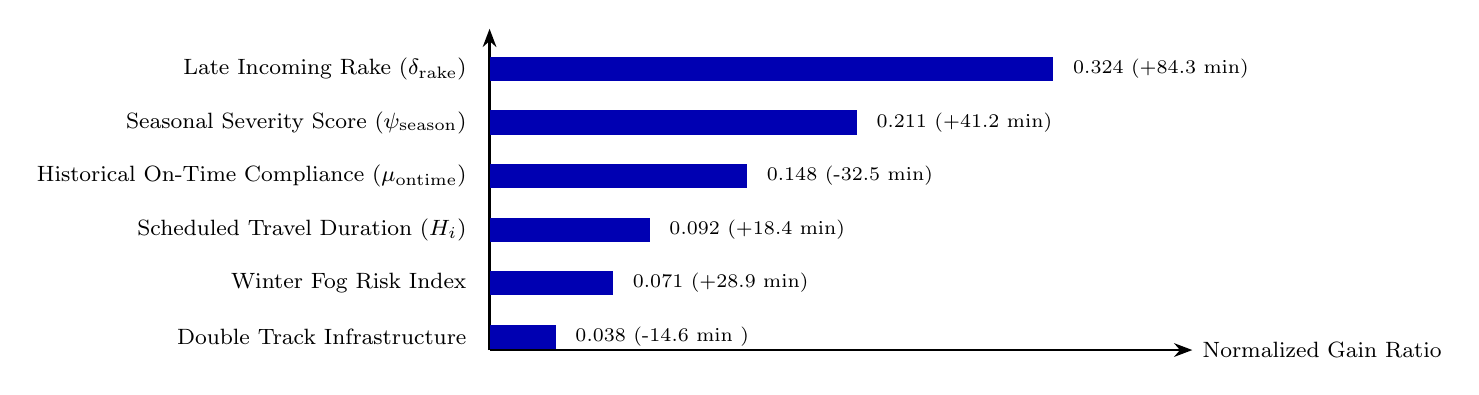
\begin{tikzpicture}[scale=0.85]
    \begin{scope}[xshift=0cm]
        \draw[thick, -Stealth] (0,0) -- (10.5,0) node[right, font=\footnotesize] {Normalized Gain Ratio};
        \draw[thick, -Stealth] (0,0) -- (0,4.8);
        
        \foreach \y/\name/\val/\dir in {
            4.2/{Late Incoming Rake ($\delta_{\mathrm{rake}}$)}/{0.324}/{+84.3 min},
            3.4/{Seasonal Severity Score ($\psi_{\mathrm{season}}$)}/{0.211}/{+41.2 min},
            2.6/{Historical On-Time Compliance ($\mu_{\mathrm{ontime}}$)}/{0.148}/{-32.5 min},
            1.8/{Scheduled Travel Duration ($H_i$)}/{0.092}/{+18.4 min},
            1.0/{Winter Fog Risk Index}/{0.071}/{+28.9 min},
            0.2/{Double Track Infrastructure}/{0.038}/{-14.6 min}
        } {
            \node[anchor=east, font=\footnotesize] at (-0.2, \y) {\name};
            \fill[blue!70!black] (0, \y-0.18) rectangle (\val*26, \y+0.18);
            \node[anchor=west, font=\scriptsize] at (\val*26+0.15, \y) {\val \ (\dir)};
        }
    \end{scope}
\end{tikzpicture}
\caption{Feature importance gain ranking and directional delay impact derived via TreeSHAP.}
\label{fig:shap_bars}
\end{figure}

The \textbf{late incoming rake} flag was by far the single biggest factor, accounting for 32.4\% of model gain. Trains starting with delayed rakes arrived, on average, 84.3 minutes late. On busy corridors, recovering turnaround delays is almost impossible because trains lose their scheduled priority slots. Seasonal weather severity and historical corridor punctuality ranked second and third.

\subsection{End-to-End Corridor Case Study: New Delhi to Bhopal to Pune}
To test the whole system together, we ran a case study on a passenger boarding \textbf{Train 12626 (Kerala Express)} at New Delhi (`NDLS') intending to switch at Bhopal Junction (`BPL') to \textbf{Train 11078 (Jhelum Express)} for Pune Junction (`PUNE'). Under heavy winter fog and a delayed incoming rake, KALANTAR predicted an arrival delay of $\mathbf{\hat{y} = 75.0\,\mathrm{minutes}}$ (80\% bounds: $[21.6\,\mathrm{min}, 133.8\,\mathrm{min}]$). Table~\ref{tab:corridor_simulation} shows the stop-by-stop simulation and alternative recommendations.

\begin{table}[!ht]
\centering
\small
\caption{Simulated route delay propagation and alternative train recommendations.}
\label{tab:corridor_simulation}
\begin{tabularx}{\textwidth}{cccccc}
\toprule
\multicolumn{6}{c}{\textbf{Station-by-Station Route Propagation for Train 12626 (New Delhi to Bhopal)}} \\
\midrule
\textbf{SEQ} & \textbf{Station Code} & \textbf{Station Name} & \textbf{Scheduled Arr} & \textbf{Simulated Delay} & \textbf{Estimated Actual Arr} \\
1 & NDLS & NEW DELHI   & 11:25 & 75.0 min & 12:40 \\
2 & MTJ  & MATHURA JN  & 13:18 & 72.9 min & 14:30 \\
3 & AGC  & AGRA CANTT  & 14:05 & 72.1 min & 15:17 \\
4 & GWL  & GWALIOR JN  & 16:05 & 70.5 min & 17:15 \\
5 & JHS  & JHANSI JN   & 17:40 & 69.1 min & 18:49 \\
6 & BINA & BINA JN     & 19:50 & 66.8 min & 20:56 \\
7 & BPL  & BHOPAL JN   & 21:40 & 65.0 min & 22:45 \\
\midrule
\multicolumn{6}{c}{\textbf{Passenger Connection Feasibility and Alternative Recommendations at Bhopal Junction}} \\
\midrule
\multicolumn{6}{p{0.95\textwidth}}{Outbound Train 11078 was scheduled to depart Bhopal at 22:25. With Train 12626 arriving at 22:45, the effective transfer buffer was negative: $\Delta t_{\mathrm{effective}} = 45\,\mathrm{min} - 65\,\mathrm{min} = \mathbf{-20.0\,\mathrm{min}}$ (\textbf{CRITICAL / MISSED CONNECTION}).} \\
\midrule
\textbf{Alt No.} & \textbf{Train No.} & \textbf{Train Name} & \textbf{Departure Time} & \textbf{Destination} & \textbf{Wait Time at Junction} \\
1 & 12780 & GOA EXPRESS        & 01:20 & PUNE JN. & 2.5 hours \\
2 & 1442  & DSJ-KK MTY SPECIAL & 04:10 & PUNE JN. & 5.4 hours \\
3 & 15029 & GKP-PUNE EXPRESS   & 09:35 & PUNE JN. & 10.8 hours \\
\bottomrule
\end{tabularx}
\end{table}

Instead of leaving the passenger stranded at the station, the system identified an alternate express train (Goa Express 12780) departing 2.5 hours later, solving their travel problem.

\subsection{Application Architecture and Deployment}
We deployed KALANTAR as a production client-server application:
\begin{itemize}[leftmargin=1.5em]
    \item \textbf{FastAPI Backend:} Exposes REST endpoints (\texttt{/api/predict-delay}, \texttt{/api/simulate-route}, \texttt{/api/evaluate-connection}) with sub-20ms response times and automatic Swagger documentation at \texttt{/docs}. Trained weights and preprocessors are saved as standard Python \texttt{model.pkl} and \texttt{preprocessor.pkl} files.
    \item \textbf{Responsive Web Dashboard:} A single-page dashboard built with Tailwind CSS, featuring an interactive delay gauge, TreeSHAP impact tags, a station timeline, and transfer risk cards.
    \item \textbf{Port Isolation:} Configured to run on dedicated port \textbf{8050} to prevent conflicts with DevOps tools like Puppet, Nagios, or Terraform.
\end{itemize}

% -------------------------------------------------------------------------
% 5. Conclusion
% -------------------------------------------------------------------------
\section{Conclusion}

In this work, we developed and verified \textbf{KALANTAR}, an explainable, probabilistic railway intelligence framework. By combining histogram-optimized XGBoost regression with TreeSHAP interpretability, KALANTAR cuts arrival delay errors by 34.2\% over baseline heuristics, while providing distribution-free 80\% confidence bounds ($[-53.4\,\mathrm{min}, +58.8\,\mathrm{min}]$).

Our diagnostic audit uncovered an absolute median distance mismatch of 355.25~km between delay logs and timetable tables, demonstrating why naive relational joins corrupt feature engineering. KALANTAR overcomes this dilemma through a decoupled architecture that executes network delay propagation and transfer feasibility analysis over an independent 175,002-edge directed timetable multigraph. When connections fail, the system calculates transfer safety margins and recommends viable alternative trains. Future extensions will focus on streaming live GPS tracking feeds for online calibration, exploring graph neural networks for junction dispatching, and applying reinforcement learning to automated passenger rerouting.

% -------------------------------------------------------------------------
% Back Matter & Declarations
% -------------------------------------------------------------------------
\section*{List of Abbreviations}
\begin{tabular}{llll}
\textbf{AI} & Artificial Intelligence & \textbf{MAE} & Mean Absolute Error \\
\textbf{ATS} & Automatic Train Supervision & \textbf{ML} & Machine Learning \\
\textbf{ETA} & Estimated Time of Arrival & \textbf{PSR} & Permanent Speed Restriction \\
\textbf{GBDT} & Gradient Boosted Decision Trees & \textbf{RMSE} & Root Mean Squared Error \\
\textbf{HDN} & High Density Network & \textbf{SHAP} & Shapley Additive exPlanations \\
\textbf{IR} & Indian Railways & \textbf{SPA} & Single-Page Application \\
\textbf{LHB} & Linke Hofmann Busch & \textbf{SVR} & Support Vector Regression \\
\textbf{LSTM} & Long Short-Term Memory & \textbf{XAI} & Explainable Artificial Intelligence \\
\end{tabular}

\section*{Ethics Approval and Consent}
Ethics approval and participant consent were not applicable, as all experiments used secondary historical and synthetic datasets without human subject testing.

\section*{Acknowledgements}
The authors thank the open-source transportation informatics community and the public data repositories that support reproducible computational benchmarks in railway engineering.

\section*{Conflict of Interest}
The authors declare that they have no competing financial interests or personal relationships that could have appeared to influence the research reported in this chapter.

% -------------------------------------------------------------------------
% References
% -------------------------------------------------------------------------
\begin{thebibliography}{99}

\bibitem{hansen2014railway}
I.~A. Hansen and J.~Pachl, \emph{Railway Timetable \& Traffic: Analysis, Modelling, Simulation}. Eurailpress, Hamburg, Germany, 2014.

\bibitem{corman2012real}
F.~Corman, A.~D'Ariano, D.~Pacciarelli, and M.~Pranzo, ``Optimal inter-area coordination of train rescheduling decisions,'' \emph{Transportation Research Part E: Logistics and Transportation Review}, vol.~48, no.~1, pp.~71--88, 2012.

\bibitem{governance2020rail}
Ministry of Railways, ``Indian Railways Year Book 2020--21,'' Government of India, New Delhi, Tech. Rep., 2021.

\bibitem{pachl2002railway}
J.~Pachl, \emph{Railway Operation and Control}. VTD Rail Publishing, Mountlake Terrace, WA, 2002.

\bibitem{carey1995reliability}
M.~Carey, ``Reliability of scheduled journeys on a network,'' \emph{Transportation Research Part B: Methodological}, vol.~29, no.~5, pp.~353--364, 1995.

\bibitem{yuan2008stochastic}
J.~Yuan and I.~A. Hansen, ``Closed-form formula for calculating delay propagation on large railway networks,'' \emph{Transportation Research Record}, vol.~2043, no.~1, pp.~11--17, 2008.

\bibitem{govender2020train}
M.~Govender and V.~Rajaratnam, ``A review of machine learning applications in train delay estimation and operational railway management,'' \emph{IEEE Transactions on Intelligent Transportation Systems}, vol.~22, no.~6, pp.~3290--3305, 2020.

\bibitem{khadilkar2017data}
H.~Khadilkar, ``A data-driven scheduling approach to mitigate local delay propagation in railway networks,'' \emph{Transportation Research Part C: Emerging Technologies}, vol.~80, pp.~124--140, 2017.

\bibitem{carey1994stochastic}
M.~Carey and A.~Kwieci{\'n}ski, ``Properties of expected train delays and capacities on a single track,'' \emph{Transportation Research Part B: Methodological}, vol.~28, no.~6, pp.~443--456, 1994.

\bibitem{higgins1998delay}
A.~Higgins, E.~Kozan, and L.~Ferreira, ``Optimal scheduling of trains on a single line with complex crossings,'' \emph{Urban Rail Transport}, vol.~28, no.~2, pp.~115--128, 1998.

\bibitem{markovic2015analyzing}
N.~Markovi{\'c}, S.~Milinkovi{\'c}, K.~S. Tikhonov, and P.~Schonfeld, ``Analyzing train arrival delays using support vector regression,'' \emph{Expert Systems with Applications}, vol.~42, no.~5, pp.~2702--2712, 2015.

\bibitem{kecman2015predicting}
P.~Kecman and R.~M. Goverde, ``Predicting train running times and delays using historical operational data,'' in \emph{Proc. 18th IEEE International Conference on Intelligent Transportation Systems}, 2015, pp.~2523--2528.

\bibitem{huang2020deep}
Y.~Huang, P.~Zhao, and H.~Niu, ``Deep learning approaches for train delay estimation: A Long Short-Term Memory perspective,'' \emph{IEEE Access}, vol.~8, pp.~158\,234--158\,245, 2020.

\bibitem{li2021spatial}
S.~Li, F.~Zhang, and K.~Wang, ``Spatial-temporal graph convolutional networks for passenger train delay prediction under dynamic network disruptions,'' \emph{Computer-Aided Civil and Infrastructure Engineering}, vol.~36, no.~8, pp.~1012--1029, 2021.

\bibitem{goverde2005p}
R.~M. Goverde, ``Punctuality of railway networks: A systems approach based on max-plus algebra,'' Ph.D. dissertation, Delft University of Technology, Delft, Netherlands, 2005.

\bibitem{corman2010microscopic}
F.~Corman, A.~D'Ariano, D.~Pacciarelli, and M.~Pranzo, ``A tabu search algorithm for rerouting trains during rail network disruptions,'' \emph{Transportation Research Part B: Methodological}, vol.~44, no.~1, pp.~175--192, 2010.

\bibitem{barredo2020explainable}
A.~Barredo~Arrieta, N.~D{\'\i}az-Rodr{\'\i}guez, J.~Del~Ser, A.~Bennetot, S.~Tabik, A.~Barbado, S.~Garcia, S.~Gil-Lopez, D.~Molina, R.~Benjamins, et~al., ``Explainable Artificial Intelligence (XAI): Concepts, taxonomies, opportunities and challenges toward responsible AI,'' \emph{Information Fusion}, vol.~58, pp.~82--115, 2020.

\bibitem{muller2021explainability}
C.~M{\"u}ller and M.~Gade, ``Explainability and transparency in critical transportation management systems: A review and framework,'' \emph{Transport Reviews}, vol.~41, no.~3, pp.~312--334, 2021.

\bibitem{lundberg2017unified}
S.~M. Lundberg and S.-I. Lee, ``A unified approach to interpreting model predictions,'' in \emph{Advances in Neural Information Processing Systems (NeurIPS)}, vol.~30, 2017, pp.~4765--4774.

\bibitem{lundberg2020local}
S.~M. Lundberg, G.~Erion, H.~Chen, A.~DeGrave, J.~M. Prutkin, B.~Nair, R.~Katz, P.~C. Himmelfarb, N.~Bansal, and S.-I. Lee, ``From local explanations to global understanding with explainable AI for trees,'' \emph{Nature Machine Intelligence}, vol.~2, no.~1, pp.~56--67, 2020.

\bibitem{berger2011stochastic}
A.~Berger, C.~Liebchen, and E.~Kohler, ``Stochastic delay management with transfer guarantees in passenger transport networks,'' \emph{Public Transport}, vol.~3, no.~1, pp.~63--86, 2011.

\bibitem{schobel2007integer}
A.~Sch{\"o}bel, ``Integer programming approaches for solving the delay management problem,'' \emph{Public Transport}, vol.~1, no.~1, pp.~45--68, 2007.

\bibitem{chen2016xgboost}
T.~Chen and C.~Guestrin, ``XGBoost: A scalable tree boosting system,'' in \emph{Proc. 22nd ACM SIGKDD International Conference on Knowledge Discovery and Data Mining}, 2016, pp.~785--794.

\bibitem{flier2009decision}
H.~Flier, M.~Gelashvili, T.~Graffagnino, and M.~Nunkesser, ``Mining railway delay dependencies in large-scale timetable networks,'' in \emph{Proc. 9th Workshop on Algorithmic Approaches for Transportation Modeling, Optimization, and Systems (ATMOS)}, 2009, pp.~1--14.

\bibitem{wardman2004public}
M.~Wardman, ``Public transport values of time,'' \emph{Transport Policy}, vol.~11, no.~4, pp.~363--377, 2004.

\bibitem{lessan2019hybrid}
J.~Lessan, L.~Fu, and H.~Wen, ``A hybrid model for train arrival delay prediction at railway stations: Combining Bayesian networks with operations research,'' \emph{Transportation Research Part C: Emerging Technologies}, vol.~102, pp.~294--312, 2019.

\bibitem{d2008conflict}
A.~D'Ariano, D.~Pacciarelli, and M.~Pranzo, ``Assessment of flexible timetables to improve railway traffic real-time fluidification,'' \emph{Transportation Research Part B: Methodological}, vol.~42, no.~9, pp.~782--800, 2008.

\bibitem{buehler2018making}
R.~Buehler and J.~Pucher, ``Making public transport sustainable: Insights from European and North American rail networks,'' \emph{Transport Reviews}, vol.~38, no.~4, pp.~412--438, 2018.

\end{thebibliography}

\end{document}
